% !TEX TS-program = xelatex
% !TeX program = xelatex
% !TEX encoding = UTF-8
% !TeX spellcheck = en_US

%=====================================================================
\ifx\wholebook\relax\else
	\documentclass{KBook}
	
\bibliographystyle{unsrtnat}%unsrtnat, plainnat

\hypersetup{
	pdfkeywords={NLP; Language},
	pdfsubject={Artificial intelligence; Natural Language Processing},
	citecolor=blue,
}



\DeclareAcronym{amr}{
	short = AMR,
	long  =  Abstract Meaning Representation,
	tag = abbrev
}

\DeclareAcronym{cfg}{
	short = CFG ,
	long  =  Context Free Grammar,
	tag = abbrev
}

\DeclareAcronym{darpa}{
	short = DARPA ,
	long  = Defense Advanced Research Projects Agency,
	tag = abbrev
}

\DeclareAcronym{edu}{
	short = EDU,
	long  = Elementary Discourse Unit,
	tag = abbrev
}

\DeclareAcronym{fol}{
	short = FOL,
	long  = First Order Logic,
	tag = abbrev
}

\DeclareAcronym{hmm}{
	short = HMM ,
	long  =  Hidden Markov Model,
	tag = abbrev
}

\DeclareAcronym{ia}{
	short = IA ,
	long  = Intelligence Artificielle,
	tag = abbrev
}

\DeclareAcronym{ibm}{
	short = IBM,
	long  = International Business Machines,
	tag = abbrev
}

\DeclareAcronym{idf}{
	short = IDF ,
	long  = Inverse Document Frequency,
	tag = abbrev
}

\DeclareAcronym{ipa}{
	short = IPA ,
	long  = Intelligent Personal Assistant,
	tag = abbrev
}

\DeclareAcronym{iva}{
	short = IVA ,
	long  = Intelligent Virtual Assistant,
	tag = abbrev
}

\DeclareAcronym{ipa2}{
	short = IPA ,
	long  =  International Phonetic Alphabet,
	tag = abbrev
}

\DeclareAcronym{lsa}{
	short = LSA,
	long  = Latent Semantic Analysis,
	tag = abbrev
}

\DeclareAcronym{memm}{
	short = MEMM ,
	long  =  Maximum Entropy Markov Model,
	tag = abbrev
}

\DeclareAcronym{ml}{
	short = ML,
	long  = Machine Learning,
	tag = abbrev
}

\DeclareAcronym{pcfg}{
	short = PCFG ,
	long  = Probabilistic Context Free Grammar,
	tag = abbrev
}

\DeclareAcronym{pdtb}{
	short = PDTB,
	long  = Penn Discourse TreeBank,
	tag = abbrev
}

\DeclareAcronym{ri}{
	short = RI,
	long  =  Recherche d'Information,
	tag = abbrev
}

\DeclareAcronym{rnn}{
	short = RNN ,
	long  = Recurrent Neural Network,
	tag = abbrev
}

\DeclareAcronym{rst}{
	short = RST,
	long  = Rhetorical Structure Theory,
	tag = abbrev
}

\DeclareAcronym{srl}{
	short = SRL,
	long  = Semantic Role Labeling,
	tag = abbrev
}

\DeclareAcronym{svd}{
	short = SVD,
	long  = Singular Value Decomposition,
	tag = abbrev
}


\DeclareAcronym{taln}{
	short = TALN,
	long  = Traitement Automatique du Langage Naturel,
	tag = abbrev
}

\DeclareAcronym{tal}{
	short = TAL ,
	long  = Traitement Automatique des Langues,
	tag = abbrev
}

\DeclareAcronym{tf}{
	short = TF ,
	long  = Term Frequency,
	tag = abbrev
}

\DeclareAcronym{tfidf}{
	short = TF-IDF ,
	long  = Term Frequency - Inverse Document Frequency,
	tag = abbrev
}

\DeclareAcronym{wsd}{
	short = WSD ,
	long  = Word Sense Disambiguation,
	tag = abbrev
}


%\makeglossaries

%\newacronym{oop}{OOP}{Object-oriented programming} 

	\begin{document}
		\mainmatter
	
\fi
%=====================================================================
\changegraphpath{../img/pos/}

\chapter{Part-of-Speech Tagging}

\begin{introduction}[NAT. L\textcolor{white}{A}NG. PROC.]
	\lettrine{A}{} word's grammatical category is a necessary feature for understanding a text. Sometimes, words can have multiple grammatical categories (natures). For example, the word "nouveau" in the phrase "C'est l'anniversaire de mon nouveau[NOUN]" does not have the same nature as in the phrase "Mon nouveau[ADJ] cours est presque terminé". This property can be even more noticeable in English, where nouns can be transformed into verbs without change (e.g., "fish"). This task is useful if we want to apply statistics on grammatical categories to improve another task, such as text classification. In this chapter, we will present the task of sequence labeling in general and morpho-syntactic tagging in particular.
\end{introduction} 

Knowing the grammatical categories of words is a step towards understanding a sentence. Let's take an example of a sentence in English: "\expword{We can can the can}". The word "can" has several meanings: (1-verb) to be able (2-verb) to put in a box (3-noun) a container. After morpho-syntactic tagging, we will have "\expword{We[pronoun] can[verb] can[verb] the[determiner] can[noun]}". It is not only useful to know the meaning of the word but also to see the structure of the sentence. Try to tag the following sentence: "\expword{Will Will will the will to Will?}". Morpho-syntactic tagging is beneficial for several tasks:
\begin{itemize}
	\item it is a preliminary step for syntactic analysis (next chapter).
	\item grammatical categories can be considered an important feature in text classification tasks. For example, the task of authorship detection can benefit from this feature; some authors use more nouns in sentences than others.
\end{itemize}


%===================================================================================
\section{Sequence Labeling}
%===================================================================================

A language can be considered a temporal phenomenon since sentences are composed of a continuous sequence of words.
Each word or set of words has linguistic features, each defining several categories.
For example, words have lexical categories: noun, verb, adjective, etc.
In general, the category of a word depends on the categories of the preceding words.
Labeling a sequence of words $w = w_1, \ldots, w_n$ is used to find an equivalent sequence of labels $t = t_1, \ldots, t_n$.

Sequence labeling can be done using manually defined rules.
One method is to assign each word a set of possible labels.
Then, rules are used to reduce the labels until reaching one label per word.
Among the rules that can be used is, for example, "A determinant is followed by a noun."
The statistical approach aims to learn annotation based on a manually annotated corpus.
The labeling problem is to maximize the conditional probability of a sequence of labels given a sequence of words (see Equation \ref{eq:es-stat}).
\begin{equation}\label{eq:es-stat}
	\hat{t} = \arg\max\limits_t P(t | w)
\end{equation}
In statistics, there are two types of models: generative and discriminative.
A generative model tries to learn the generation of the input from the output; given a label, what is the probability of each word in the vocabulary?
Using Bayes' theorem, Equation \ref{eq:es-stat} is equivalent to solving Equation \ref{eq:es-stat-gen}.
The Hidden Markov Model, or HMM, is an example of a generative model.
\begin{equation}\label{eq:es-stat-gen}
	\hat{t} = \arg\max\limits_t P(t) P(w | t) 
\end{equation}
Unlike generative models, a discriminative model directly estimates the probability $P(t | w)$.
This involves learning the label of a word based on its features plus the features of a limited number of words before.
A model that follows this method is the Maximum Entropy Markov Model (MEMM).
Another method is to use recurrent neural networks that support the temporal aspect.

Part of sequence labeling tasks is morpho-syntactic labeling.
Its goal is to find the grammatical categories of words (noun, verb, etc.) in a sentence.
Sometimes, we want to detail the categories for more precision.
For example, a noun can be a proper noun or a common noun.
An example of a morpho-syntactically labeled sentence in English is shown in Figure \ref{fig:ems-exp}.
\begin{figure}[ht]
	\centering
	\hgraphpage[.8\textwidth]{exp-pos2_.pdf}
	\caption[Example of morpho-syntactic labeling.]{Example of morpho-syntactic labeling by \url{https://corenlp.run/} [visited on 2022-05-19].}
	\label{fig:ems-exp}
\end{figure}

Another task of this type is named entity recognition.
It aims to find people, organizations, places, numbers, etc. in a sentence.
Unlike morpho-syntactic labeling, a category can be assigned to a sequence of words and not just one.
For example, the expression "\expword{école nationale supérieure d'informatique}" has the category "organization."
But how can we express that all these words form a single category and not each word separately?
The method used for this is the \textit{Inside, Outside, Beginning} (IOB) format.
Words that do not belong to any category are labeled as "O."
Words that mark the beginning of a category are labeled as "B-" followed by the name of the category.
Words in the middle are labeled as "I-" followed by the name of the category.
So, the previous expression will be labeled as "\expword{école[B-ORG] nationale[I-ORG] supérieure[I-ORG] d'informatique[I-ORG].}"
Figure \ref{fig:ner-exp} represents an example of a sentence in English containing named entities.
\begin{figure}[ht]
	\centering
	\hgraphpage[.8\textwidth]{exp-ner2_.pdf}
	\caption[Example of named entity recognition.]{Example of named entity recognition by \url{https://corenlp.run/} [visited on 2022-05-19].}
	\label{fig:ner-exp}
\end{figure}

Surface syntactic analysis (Chunking) is another example of sequence labeling.
It aims to find the phrases of a sentence without a tree structure.
So, the category is assigned to a sequence and not just a single word.


%===================================================================================
\section{Resources for Morpho-Syntactic Tagging}
%===================================================================================

As mentioned before, this task aims to find the grammatical category of each word in a sentence.
A grammatical category may have several names (according to the source): nature, lexical category, grammatical class, grammatical species, part of speech.
To perform this task, we must first define the tags.
Do we detail the categories, or do we stick to the main categories?
The most famous tags are those of the Penn TreeBank for English: coordinating conjunction (CC), cardinal number (CD), determiner (DT), etc.
Grammatical categories vary from one language to another, but some categories are shared.
The "Universal Dependencies" project seeks to standardize these categories, as shown in Table \ref{tab:pos-cat}.

\begin{table}[ht]
	\centering
	%	\footnotesize
	\begin{tabular}{lll}
		\hline\hline
		\textbf{Open Class} & \textbf{Closed Class} & \textbf{Others} \\
		\hline%\hline
		\keyword{ADJ}: adjective & \keyword{ADP}: adposition & \keyword{PUNCT}: punctuation \\
		%	\hline
		\keyword{ADV}: adverb & \keyword{AUX}: auxiliary & \keyword{SYM}: symbol \\
		%	\hine
		\keyword{INTJ}: interjection & \keyword{CCONJ}: coordinating conjunction & \keyword{X}: Others \\
		%	\hline
		\keyword{NOUN}: noun & \keyword{DET}: determiner &  \\
		%	\hline
		\keyword{PROPN}: proper noun & \keyword{NUM}: numeric &  \\
		%	\hline
		\keyword{VERB}: verb & \keyword{PART}: particle &  \\
		%	\hline
		& \keyword{PRON}: pronoun &  \\
		%	\hline
		& \keyword{SCONJ}: subordinating conjunction &  \\
		\hline\hline
		
	\end{tabular}
	\caption[Universal grammatical categories]{Universal grammatical categories according to \url{https://universaldependencies.org/u/pos/} [visited on 2021-09-25] \label{tab:pos-cat}}
\end{table}

The next step is to annotate a corpus manually.
This type of corpus is called a TreeBank.
Among annotated corpora, we can mention the Penn Treebank for English (Example in Figure \ref{fig:penn-exp}).
Another project rich in terms of processed languages is the Universal TreeBank\footnote{Universal TreeBank: \url{https://universaldependencies.org/} [visited on 2021-09-09]} \cite{2012-petrov-al}.
It is an open community project that aims to use the same grammatical classes to annotate multiple languages.
However, caution is needed when merging two different treebanks.
When there are multiple tags, inconsistencies in the annotation may arise.
For example, in the "Brown" and "WSJ" corpora, the word "to" has the tag "TO."
In the "Switchboard" corpus, it has the tag "TO" when indicating the infinitive, otherwise "IN" when it is a preposition.

\begin{figure}[ht]
	\centering
	\begin{tcolorbox}[colback=white, colframe=blue, boxrule=1pt, text width=.62\textwidth]
		\footnotesize
		\begin{alltt}
			Battle-tested\keyword{/JJ} Japanese\keyword{/JJ} industrial\keyword{/JJ} managers\keyword{/NNS}
			here\keyword{/RB} always\keyword{/RB} buck\keyword{/VBP} up\keyword{/RP} nervous\keyword{/JJ} newcomers\keyword{/NNS}
			with\keyword{/IN} the\keyword{/DT} tale\keyword{/NN} of\keyword{/IN} the\keyword{/DT} first\keyword{/JJ} of\keyword{/IN}
			their\keyword{/PP\$} countrymen\keyword{/NNS} to\keyword{/TO} visit\keyword{/VB} Mexico\keyword{/NNP} ,\keyword{/,}
			a\keyword{/DT} boatload\keyword{/NN} of\keyword{/IN} samurai\keyword{/FW} warriors\keyword{/NNS} blown\keyword{/VBN}
			ashore\keyword{/RB} 375\keyword{/CD} years\keyword{/NNS} ago\keyword{/RB} .\keyword{/.}
		\end{alltt}
	\end{tcolorbox}
	\caption[Example of a Penn TreeBank annotated text.]{Example of a Penn TreeBank annotated text; figure reconstructed from \cite{2003-taylor}.}
	\label{fig:penn-exp}
\end{figure}

Here are some applications that provide morpho-syntactic tagging:
\begin{itemize}
	\item \url{https://nlp.stanford.edu/software/tagger.shtml} [visited on 2021-09-26]
	\item \url{https://github.com/sloria/textblob} [visited on 2021-09-26]
	\item \url{https://www.nltk.org/api/nltk.tag.html} [visited on 2021-09-26]
	\item \url{https://spacy.io/} [visited on 2021-09-26]
	\item \url{https://github.com/clips/pattern} [visited on 2021-09-26]
\end{itemize}


%===================================================================================
\section{Morpho-Syntactic Tagging Approaches}
%===================================================================================

Here, we will only present the statistical and neural approaches. In the statistical approach, we will introduce the Hidden Markov Model, which is a generative model, and the Maximum Entropy Markov Model, which is a discriminative model. In the neural-based approach, we will present some architectures.

\subsection{Hidden Markov Model}

Given a sequence of state variables $q_1, \ldots, q_i$, the Markov assumption (as seen in the previous chapter) states that the probability of being in a state depends only on the previous state. Thus, $P(q_i | q_1, \ldots, q_{i-1}) \approx P(q_i | q_{i-1})$. A Markov chain can be formalized as a set of states $Q = \{q_1, q_2, \ldots, q_n\}$, an initial distribution of probabilities $\pi = [\pi_1, \pi_2, \ldots, \pi_n ],\, \sum_i \pi_i = 1$, and a matrix of transition probabilities
$
A = \begin{bmatrix}%
	a_{11} & a_{12} & \ldots & a_{1n} \\
	a_{21} & a_{22} & \ldots & a_{2n} \\
	\vdots & \vdots & \ddots & \vdots \\
	a_{n1} & a_{n2} & \ldots & a_{nn} \\
\end{bmatrix}
$

Figure \ref{fig:cm-exp} shows an example of a Markov chain for weather prediction. It is clear that the states are $Q = [H, C, W]$ (Hot, Cold, Warm). If we assume that the initial distribution is $\pi = [0.1, 0.7, 0.2]$, the probability of the sequence $H\, W\, C\, C$ would be calculated as follows:
\begin{align*}
	P(H\, W\, C\, C) & = P(H) P(W | H) P(C | H\, W) P(C | H\, W\, C) \\
	& = \pi(H) P(W | H) P(C | W) P(C | C) \\
	& = 0.1 * 0.3 * 0.1 * 0.8 \\
\end{align*}

\begin{figure}[ht]
	\centering
	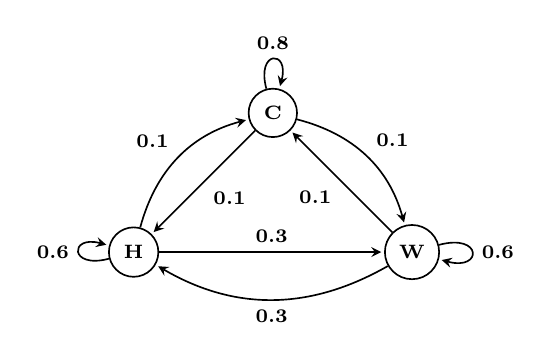
\begin{tikzpicture}[
		> = stealth, % arrow head style
		shorten > = 1pt, % don't touch arrow head to node
		auto,
		node distance = 2.5cm, % distance between nodes
		semithick, % line style
		font=\scriptsize\bfseries
		]
		
		\node[circle,draw] (qC) {C};
		\node[circle,draw] (qH) [below left of=qC] {H};
		\node[circle,draw] (qW) [below right of=qC] {W};
		
		\path[->] 	
		(qC) 	edge [loop above] node {0.8} ()
		edge [] node {0.1} (qH)
		edge [bend left] node {0.1} (qW)
		(qH) 	edge [loop left] node {0.6} ()
		edge [bend left] node {0.1} (qC)
		edge [] node {0.3} (qW)
		(qW)	edge [loop right] node {0.6} ()
		edge [bend left] node {0.3} (qH)
		edge [] node {0.1} (qC);
	\end{tikzpicture}
	\caption[Example of a Markov chain for weather prediction.]{Example of a Markov chain for weather prediction; figure reconstructed from \cite{2019-jurafsky-martin}.}
	\label{fig:cm-exp}
\end{figure}


%\begin{figure}[ht]
%	\centering
%	\hgraphpage[.4\textwidth]{exp-markov_.pdf}
%	\caption[Exemple d'un chaîne de Markov pour la prédiction du temps]{Exemple d'un chaîne de Markov pour la prédiction du temps \cite{2019-jurafsky-martin}\label{fig:cm-exp}}
%\end{figure}

This is a language model that represents only transition probabilities. In this case, we can only represent the transition probability from one category to another. If we estimate the emission probability of a word in each state (label), we could estimate the labels using Bayes' theorem. This model is called the Hidden Markov Model (\ac{hmm}); the words in a sequence are observed, unlike the hidden categories that need to be estimated. Each label (category) $t_i$ is represented by a state $q_i$ in the set of states $Q = \{q_1, q_2, \ldots, q_n\}$. Transitions from one state to another following a Bigram model are represented by the transition matrix $A$. The initial distribution of probabilities for these states is denoted $\pi = [\pi_1, \pi_2, \ldots, \pi_n]$, where $\sum_i \pi_i = 1$. A word $w_i$ is represented as an observation in the sequence of observed events $O = o_1 o_2 \ldots o_T$. An observation $o_t$ can be generated in a state $q_i$ with observation probabilities (emission probabilities) $B = b_i(o_t)$. An example of an \ac{hmm} is illustrated in Figure \ref{fig:hmm-exp}. Transitions represent the probabilities of moving from one label to another. Emissions represent the probabilities of word occurrences in labels.
\begin{figure}[ht]
	\centering
	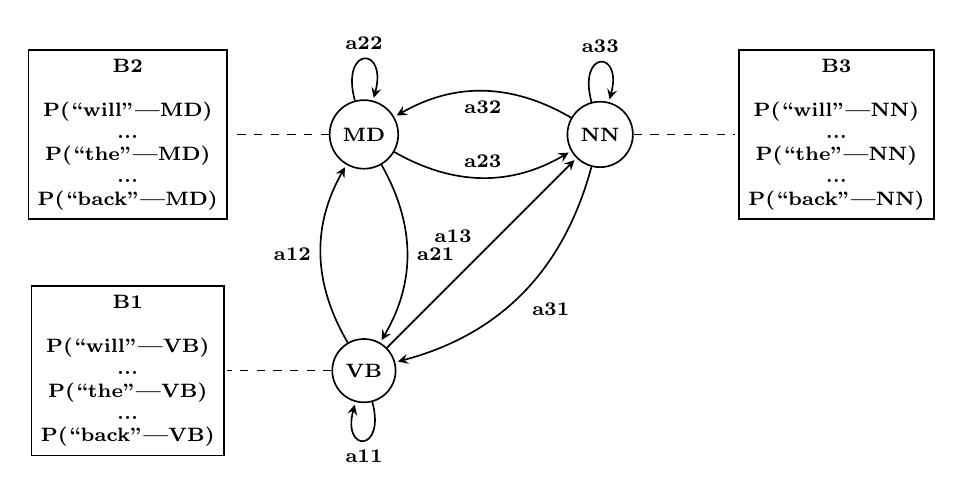
\begin{tikzpicture}[
		> = stealth, % arrow head style
		shorten > = 1pt, % don't touch arrow head to node
		auto,
		node distance = 3cm, % distance between nodes
		semithick, % line style
		font=\scriptsize\bfseries
		]
		
		\node[circle,draw] (q2) {MD};
		\node[align=center,draw] (q2e) [left of=q2] {B2\\ \\P(``will"|MD)\\...\\P(``the"|MD)\\...\\P(``back"|MD)};
		\node[circle,draw] (q3) [right of=q2] {NN};
		\node[align=center,draw] (q3e) [right of=q3] {B3\\ \\P(``will"|NN)\\...\\P(``the"|NN)\\...\\P(``back"|NN)};
		\node[circle,draw] (q1) [below of=q2] {VB};
		\node[align=center,draw] (q1e) [left of=q1] {B1\\ \\P(``will"|VB)\\...\\P(``the"|VB)\\...\\P(``back"|VB)};
		
		\path[->] 	
		(q1) 	edge [loop below] node {a11} ()
		edge [bend left] node {a12} (q2)
		edge [] node {a13} (q3)
		(q2) 	edge [loop above] node {a22} ()
		edge [bend left] node {a21} (q1)
		edge [bend right] node {a23} (q3)
		(q3)	edge [loop above] node {a33} ()
		edge [bend left] node {a31} (q1)
		edge [bend right] node {a32} (q2);
		
		\path[dashed] 	
		(q1) 	edge [] node {} (q1e)
		(q2) 	edge [] node {} (q2e)
		(q3) 	edge [] node {} (q3e);
		
	\end{tikzpicture}
	\caption[Example of HMM Representation]{Example of HMM Representation; figure reconstructed from \cite{2019-jurafsky-martin}.}
	\label{fig:hmm-exp}
\end{figure}

%\begin{figure}[ht]
%	\centering
%	\hgraphpage[.6\textwidth]{exp-hmm_.pdf}
%	\caption[Exemple d'une représentation HMM]{Exemple d'une représentation HMM \cite{2019-jurafsky-martin}\label{fig:hmm-exp}}
%\end{figure}

The estimated sequence $\hat{t}$ is the one that maximizes the probability $P(t)$ and the probability $P(w | t)$ according to Equation \ref{eq:hmm-detail}. Using a Bigram model, the probability $P(t)$ is calculated using transitions from the initial state $t_1$ to the last state $t_n$. It is important to note that the probability $P(t_1|t_0)$ is actually the initial probability $\pi_1$ of state $t_1$. The probability $P(w_i | t_i)$ is an emission probability in the Hidden Markov Model.

\begin{align}
	\hat{t} & = \arg\max\limits_t P(t) P(w | t) \nonumber\\
	& = \arg\max\limits_t P(t_1 \dots t_n) P(w_1 \dots w_n | t_1 \dots t_n) \nonumber\\
	& = \arg\max\limits_t \pi_{t1} \prod_{i=2}^{n} P(t_i|t_{i-1}) \prod_{i=1}^{n} P(w_i| t_i) \nonumber\\
	& = \arg\max\limits_t \prod_{i=1}^{n} \underbrace{P(t_i|t_{i-1})}_{a_{i-1,i}} \underbrace{P(w_i | t_i)}_{b_i(w_i)} \label{eq:hmm-detail}
\end{align}

Before discussing how a sequence $w=w_1 \ldots w_n$ is decoded according to Equation \ref{eq:hmm-detail}, we begin by describing training. In an \ac{hmm}, the states are the tags (categories) $t_i$, and the observations are the words $w_i$. Let the function that counts the occurrences of a sequence be denoted as $C$. The transition probability $a_{i-1,i}$ from state $t_{i-1}$ to $t_i$ is estimated from the training corpus according to Equation \ref{eq:pos-hmm1}. Note "<s>" is the label preceding the first category of the sentence. In this case, the probability $\pi_i$ of starting with state $t_i$ is estimated according to Equation \ref{eq:pos-hmm2}. The emission probability of a word $w_i$ in a state $t_i$ is estimated according to Equation \ref{eq:pos-hmm3}.

\begin{align}
	P(t_i | t_{i-1}) & = \frac{C(t_{i-1}, t_i)}{C(t_{i-1})}  \label{eq:pos-hmm1} \\
	\pi_i & = P(t_i | <s>) = \frac{C(<s>, t_i)}{C(<s>)} \label{eq:pos-hmm2} \\
	P(w_i | t_i) & = \frac{C(t_i, w_i)}{C(t_i)} \label{eq:pos-hmm3}
\end{align}

Let's take an example of a training corpus with four sentences and four categories: DT, PR, VB, and NM.

\begin{itemize}
	\item un/DT ordinateur/NM peut/VB vous/PR aider/VB
	\item il/PR veut/VB vous/PR aider/VB
	\item il/PR veut/VB un/DT ordinateur/NM
	\item il/PR peut/VB nager/VB
\end{itemize}

An example of calculating a transition is as follows: $P(VB | NM) = \frac{C(NM,\ VB)}{C(NM)} = \frac{1}{2}$. The emission probability of the word "veut" when the tag is "VB" is calculated as follows: $P(veut | VB) = \frac{C(VB,\ veut)}{C(VB)} = \frac{2}{7}$. The probability of a pronoun being at the beginning of the sentence is calculated as: $\pi_{PR} = \frac{C(<s>,\ PR)}{C(<s>)} = \frac{3}{4}$. The transition matrix as well as the initial distribution are illustrated in Table \ref{tab:hmm-trans-init}. Even though it is not used in the calculation, we added the transition from one state to the end to complete the distribution (to have a sum of 1 on the rows). Emission probabilities are illustrated in Table \ref{tab:hmm-emission}.

\begin{table}[ht]
	\centering\footnotesize
	\begin{tabular}{llllll}
		\cline{2-6}\noalign{\vskip\doublerulesep
			\vskip-\arrayrulewidth}\cline{2-6}
		& DT & PR & VB & NM & \textless/s\textgreater\\
		\hline
		DT  &  0  &  0   &  0   &   1  &  0  \\
		PR &  0  &  0   &   1  &  0   &  0  \\
		VB & 1/7 & 2/7  & 1/7  &  0   & 3/7 \\
		NM &  0  &  0   & 1/2  &   0  &  1/2 \\
		\hline
		\textless s\textgreater ($\pi$) &  1/4  &  3/4   & 0  &   0  &  0 \\
		\hline\hline
	\end{tabular}
	\caption[Example of transition probabilities and an initial distribution]{Example of transition probabilities and an initial distribution \label{tab:hmm-trans-init}}
\end{table}

\begin{table}[ht]
	\centering\footnotesize
	\begin{tabular}{lllllllll}
		\cline{2-9}\noalign{\vskip\doublerulesep
			\vskip-\arrayrulewidth}\cline{2-9}
		& un & ordinateur & peut & vous & aider & il & veut & nager \\
		\hline
		DT  &  1 &  0         &  0   &   0  &  0    & 0  & 0    & 0 \\
		PR &   0 &  0         &  0   & 1/4  &  0    &3/4 & 0    & 0 \\
		VB &   0 &  0         & 2/7  &   0  &  2/7  & 0  & 2/7  & 1/7 \\
		NM &   0 &  1         &  0   &   0  &  0    & 0  & 0    & 0 \\
		\hline\hline
	\end{tabular}
	\caption[Example of emission probabilities]{Example of emission probabilities \label{tab:hmm-emission}}
\end{table}

%\begin{figure}
%	\begin{tikzpicture}[
%	> = stealth, % arrow head style
%	shorten > = 1pt, % don't touch arrow head to node
%	auto,
%	node distance = 3cm, % distance between nodes
%	semithick, % line style
%	font=\small
%	]
%	
%	\tikzstyle{every state}=[
%	draw = black,
%	thick,
%	fill = white,
%	minimum size = 4mm
%	]
%	
%	\node[circle,draw] (qN) {N};
%	\node[align=left,draw] (qNe) [left of=qN] {P("fish"|N)=0.05\\P("river"|N)=0.03};
%	\node[circle,draw] (qV) [right of=qN] {V};
%	\node[align=left,draw] (qVe) [right of=qV] {P("fish"|V)=0.01\\P("eat"|V)=0.02};
%	\node[circle,draw] (qD) [below of=qN] {D};
%	\node[align=left,draw] (qDe) [left of=qD] {P("the"|D)=0.3\\P("a"|D)=0.2\\P("an"|D)=0.15};
%	\node[circle,draw] (qP) [right of=qD] {P};
%	\node[align=left,draw] (qPe) [right of=qP] {P("I"|P)=0.2\\P("he"|P)=0.1\\P("she"|P)=0.1};
%	\node[] () [below of=qD, yshift=1.5cm] {$\pi(P, D, V, N) = (0.4, 0.3, 0.1, 0.2)$};
%	
%	
%	\path[->] 	
%	(qN) 	edge [loop above] node {0.3} ()
%	edge [bend left] node {0.7} (qV)
%	(qV) 	edge [loop above] node {0.1} ()
%	edge [bend left] node {0.5} (qN)
%	edge [bend left] node {0.4} (qD)
%	(qD)	edge [bend left] node {1.0} (qN)
%	(qP)	edge [bend right] node {1.0} (qV);
%	
%	\path[dashed] 	
%	(qN) 	edge [] node {} (qNe)
%	(qV) 	edge [] node {} (qVe)
%	(qD) 	edge [] node {} (qDe)
%	(qP) 	edge [] node {} (qPe);
%	
%	\end{tikzpicture}
%	\caption{Exemple}
%\end{figure}

Now let's go back to the decoding of tags (tagging). After training a Hidden Markov Model $\lambda = (A, B)$, we want to use it to estimate the tag sequence $\hat{t} = \hat{t}_1 \hat{t}_2 \ldots \hat{t}_T$ from a sequence of observations (words) $w = w_1 w_2 \ldots w_T$ where we have $N$ possible tags. If we were to use a brute force decoding, we would have a complexity of $O(N^T)$. Since maximizing the tags for an observation (word) $w_t$ depends only on the tags of the previous observation, we can solve the search problem using dynamic programming. At each step $t$ of the sequence, we rely on the previous estimation to compute the probabilities of all tags in order to choose the one that maximizes the probability as the current estimation. We always need to save the previous state to go back at the end of the algorithm. This is called the \textbf{Viterbi} search (see Algorithm \ref{algo:viterbi}). In this case, the complexity is reduced to $O(N^2T)$, and the search remains exact.

\begin{algorithm}[ht]
	\KwData{$w = w_1 \ldots w_T$, HMM $\lambda = (A, B)$ with $N$ states}
	\KwResult{$best\_path$, $prob\_path$}
	
	Create two matrices $viterbi[N, T]$ and $backpointer[N, T]$\;
	
	\For{state $ s = 1 \ldots N$}{
		$viterbi[s, 1] = \pi_s * b_s(w_1);\, backpointer[s, 1] = 0$ \;
	}
	
	\For{$ t = 2 \ldots T$}{
		\For{state $ s = 1 \ldots N$}{
			$viterbi[s, t] = \max\limits_{s'=1}^N viterbi[s', t-1] * a_{s',s} * b_s(w_t)$\;
			$backpointer[s, t] = \arg\max\limits_{s'=1}^N viterbi[s', t-1] * a_{s',s} * b_s(w_t)$\;
		}
	}
	
	$prob\_path = \max\limits_{s=1}^N viterbi[s, T];\, pointer\_path = \arg\max\limits_{s=1}^N viterbi[s, T]$\;
	
	$best\_path$ is the path starting from $pointer\_path$ and following $backpointer$
	
	\Return $best\_path$, $prob\_path$\;
	\caption{Viterbi Algorithm for decoding a sequence according to a Hidden Markov Model.}
	\label{algo:viterbi}
\end{algorithm}

Using the trained model in the previous example, we want to find the tags for this sentence: \expword{il peut aider}. According to the Viterbi algorithm, we will have Table \ref{tab:hmm-viterbi-exp} where each cell is filled with calculations separated by semicolons (previous states) and the return pointer between square brackets. In the last sequence ("aider"), the state that maximizes the probability is "VB". The return is state 3 ("VB") with a return to state 2 ("PR"). Therefore, the annotated text is: \expword{il/PR peut/VB aider/VB}.


%\begin{table}[ht]
%	\centering\small
%	\begin{tabular}{llll}
%		\cline{2-4}\noalign{\vskip\doublerulesep
%			\vskip-\arrayrulewidth}\cline{2-4}
%		       & il & peut & aider \\
%		\hline
%		\multirow{4}{*}{DET}  &  \multirow{4}{*}{1/4 * 0}& 0 * 0 * 0 & 0 * 0 * 0 \\
%		  &  & 3/4 * 0 * 0 & 0 * 0 * 0\\
%		  &  & 0 * 1/7 * 0 & 6/28 * 1/7 * 0 \\
%		  &  & 0 * 0 * 0 & 0 * 0 * 0\\
%		\multirow{4}{*}{PRON} &  \multirow{4}{*}{3/4 * 1} &  0 * 0 * 0&  0 * 0 * 0\\
%		  &  & 3/4 * 0 * 0 & 0 * 0 * 0\\
%		  &  & 0 * 2/7 * 0 & 6/28 * 2/7 * 0\\
%		  &  & 0 * 0 * 0 & 0 * 0 * 0 \\
%		\multirow{4}{*}{VERB} &  \multirow{4}{*}{0 * 0} & 0 * 0 * 2/7 & 0 * 0 * 2/7 \\
%		  &  & 3/4 * 1 * 2/7 & 0 * 1 * 2/7 \\
%		  &  & 0 * 1/7 * 2/7 & 6/28 * 1/7 * 2/7\\
%		  &  & 0 * 1/2 * 2/7 & 0 * 1/7 * 2/7 \\
%		\multirow{4}{*}{NOUN} &  \multirow{4}{*}{0 * 0} & 0 * 1 * 0 & 0 * 1 * 0 \\
%		  &  & 3/4 * 0 * 0 & 6/28 * 0 * 0 \\
%		  &  & 0 * 0 * 0 & 0 * 0 * 0 \\
%		  &  & 0 * 0 * 0 & 0 * 0 * 0\\
%		\hline\hline
%	\end{tabular}
%	\caption{Un exemple des probabilités d'émission \label{tab:hmm-viterbi-exp}}
%\end{table}

\begin{table}[ht]
	\centering\footnotesize%\scriptsize
	\begin{tabular}{llll}
		\cline{2-4}\noalign{\vskip\doublerulesep
			\vskip-\arrayrulewidth}\cline{2-4}
		& il & peut & aider \\
		\hline
		DT  & $\frac{1}{4} * 0$ [0]& $0 * 0 * 0$; $\frac{3}{4} * 0 * 0$; $0 * \frac{1}{7} * 0$; $0 * 0 * 0$ [2] & $0 * 0 * 0$; $0 * 0 * 0$; $\frac{6}{28} * \frac{1}{7} * 0$; $0 * 0 * 0$ [3]\\
		PR & $\frac{3}{4} * 1$ [0]&  $0 * 0 * 0$; $\frac{3}{4} * 0 * 0$; $0 * \frac{2}{7} * 0$; $0 * 0 * 0$ [2]&  $0 * 0 * 0$; $0 * 0 * 0$; $\frac{6}{28} * \frac{2}{7} * 0$; $0 * 0 * 0$ [3]\\
		VB & $0 * 0$ [0]& $0 * 0 * \frac{2}{7}$; $\frac{3}{4} * 1 * \frac{2}{7}$; $0 * \frac{1}{7} * \frac{2}{7}$; $0 * \frac{1}{2} * \frac{2}{7}$ [2]& $0 * 0 * \frac{2}{7}$; $0 * 1 * \frac{2}{7}$; $\frac{6}{28} * \frac{1}{7} * \frac{2}{7}$; $0 * \frac{1}{7} * \frac{2}{7}$ [3]\\
		NM & $0 * 0$ [0]& $0 * 1 * 0$; $\frac{3}{4} * 0 * 0$; $0 * 0 * 0$; $0 * 0 * 0$ [1]& $0 * 1 * 0$; $\frac{6}{28} * 0 * 0$; $0 * 0 * 0$; $0 * 0 * 0$ [1]\\
		\hline\hline
	\end{tabular}
	\caption[Exemple d'exécution de l'algorithme de Viterbi]{Exemple d'exécution de l'algorithme de Viterbi \label{tab:hmm-viterbi-exp}}
\end{table}


%===================================================================================
\subsection{Maximum Entropy}
%===================================================================================

Estimates by Hidden Markov Models (\ac{hmm}) rely only on word statistics. It is difficult to introduce features such as suffixes, uppercase letters, etc. Logistic regression, which is a discriminative model, can combine several features to estimate an output probability. Unfortunately, this method does not take sequences into consideration. We can use features on the current word and the preceding words to estimate the label, as in Hidden Markov Models (\ac{hmm}). In this case, the model will be called a \acf{memm}. The problem comes down to maximizing the individual probabilities of each label $\hat{t}_i$ (see Equation \ref{eq:pos-emm-est}).
\begin{equation}\label{eq:pos-emm-est}
	\hat{t} = \arg\max\limits_t P(t | w) = \arg\max\limits_t \prod\limits_{i} P(t_i | w_i, t_{i-1})
\end{equation}
Let $s_i^j$ be the sequence $s_i \ldots s_j$. To estimate the label $t_i$ of a word $w_i$, we take $l$ previous words and $l$ subsequent words, in addition to $k$ previous tags. We use a set of features $f$ where $f_j$ can be the presence of uppercase letters in the word, etc. Using logistic regression, the problem will be formulated as in Equation \ref{eq:memm}. Learning aims to minimize the sum of multi-class labeling errors for each word (for each word, we will have several probabilities; one for each label).
\begin{equation}\label{eq:memm}
	\hat{t} = \arg\max\limits_t \prod\limits_{i}  
	\frac{exp\left(\sum_j \theta_j f_j(t_i, w_{i-l}^{i+l}, t_{i-k}^{i-1})\right)}%
	{\sum_{t' \in tags} exp\left(\sum_j \theta_j f_j(t'_i, w_{i-l}^{i+l}, t_{i-k}^{i-1})\right)}
\end{equation}

Here is a list of features $f$ that we can use in this method:
\begin{itemize}
	\item The word $w_i$ (considering each word as a feature)
	\item Previous tags
	\item $w_i$ contains a prefix from a list (\textit{len(prefix)} $\le 4$)
	\item $w_i$ contains a suffix from a list (\textit{len(suffix)} $\le 4$)
	\item $w_i$ contains a number
	\item $w_i$ contains an uppercase letter
	\item $w_i$ contains a hyphen
	\item $w_i$ is entirely in uppercase
	\item The shape of the word $w_i$ (Ex. \expword{X.X.X})
	\item $w_i$ is in uppercase with a hyphen and a number (Ex. \expword{CFC-12})
	\item $w_i$ is in uppercase followed by the words Co., Inc., etc. within 3 words maximum
\end{itemize}

\subsection{Neural network}

Recurrent Neural Networks (\ac{rnn}) are designed to process sequences. We have seen that an \ac{rnn} can be used as a language model by inputting the encoded word with \keyword[O]{One-Hot} and estimating the next word given the previous context. We modify the output: instead of the probabilities of words in the vocabulary, we try to estimate the probabilities of possible categories. Of course, we can use a hidden layer to learn a more compact representation of words in the input (\keyword[E]{embedding}). Figure \ref{fig:pos-rnn1} represents an example of a recurrent neural network for morpho-syntactic tag detection following this modification.
\begin{figure}[ht]
	\centering
	\hgraphpage[.6\textwidth]{rnn-simple.pdf}
	\caption[RNN simple pour l'étiquetage morpho-syntaxique.]{RNN simple pour l'étiquetage morpho-syntaxique.}
	\label{fig:pos-rnn1}
\end{figure}
%\begin{figure}[!ht]
%	\centering
%	\hgraphpage[.55\textwidth]{rnn-simple_.pdf}
%	\caption[RNN simple pour l'étiquetage morpho-syntaxique]{RNN simple pour l'étiquetage morpho-syntaxique \cite{2019-jurafsky-martin}\label{fig:pos-rnn1}}
%\end{figure}

If we wanted deeper and more complex networks, we could stack multiple \ac{rnn}s together. This allows the model to learn more complex processes, improving prediction. To train this model, we will need a large dataset; the size of this dataset increases with the number of stacked networks. Figure \ref{fig:pos-rnn2} illustrates a model with two stacked \ac{rnn}s.
\begin{figure}[ht]
	\centering
	\hgraphpage[.7\textwidth]{rnn-stack.pdf}
	\caption[RNNs empilés pour l'étiquetage morpho-syntaxique.]{RNNs empilés pour l'étiquetage morpho-syntaxique.}
	\label{fig:pos-rnn2}
\end{figure}
%\begin{figure}[!ht]
%	\centering
%	\hgraphpage[.55\textwidth]{rnn-stack_.pdf}
%	\caption[RNNs empilés pour l'étiquetage morpho-syntaxique]{RNNs empilés pour l'étiquetage morpho-syntaxique \cite{2019-jurafsky-martin}\label{fig:pos-rnn2}}
%\end{figure}

In the previous neural models, the current label $t_i$ depends on the current word $w_i$ and the past context. Sometimes, knowing the future context can improve the current decision; we can find a dependence between the current word and the words that follow. To estimate the current label based on the future context, we use a \ac{rnn} with a reversed sequence; that is, the label $t_i$ will depend on the sequence $w_n, w_{n-1}, \ldots, w_{i+1}, w_{i}$. To express bidirectionality, we use two \ac{rnn}s: forward $RNN_{forward}(w_1^i)$ and backward $RNN_{backward}(w_i^n)$. We calculate the sum between the two hidden states $h_i^f \oplus h_i^b$, resulting in a vector that must pass through a "softmax" function to estimate the tag probabilities. This architecture is illustrated in Figure \ref{fig:pos-rnn3}.
\begin{figure}[ht]
	\centering
	\hgraphpage[.7\textwidth]{rnn-bi.pdf}
	\caption[RNN bidirectionnel pour l'étiquetage morpho-syntaxique.]{RNN bidirectionnel pour l'étiquetage.}
	\label{fig:pos-rnn3}
\end{figure}
%\begin{figure}[!ht]
%	\centering
%	\hgraphpage[.60\textwidth]{rnn-bi_.pdf}
%	\caption[RNN bidirectionnel pour l'étiquetage morpho-syntaxique]{RNN bidirectionnel pour l'étiquetage morpho-syntaxique \cite{2019-jurafsky-martin}\label{fig:pos-rnn3}}
%\end{figure}

Languages are always evolving: adding new words, new forms, etc. In addition, we cannot capture all the variations of all words using a limited corpus, especially in strongly inflected languages. To represent the morphological variations of a word, we have to go down to the character level. An idea (see Figure \ref{fig:pos-rnn4}) is to use a character-level language model to encode a word and combine this code with the lexical code (\keyword[O]{One-Hot} or \keyword[E]{embedding}) of the word. The resulting code will be taken as the input of the recurrent network (simple, stacked, or bidirectional).
\begin{figure}[ht]
	\centering
	\hgraphpage[0.8\textwidth]{rnn-char.pdf}
	\caption[Embedding de caractères pour l'étiquetage morpho-syntaxique.]{RNN avec des embedding de caractères pour l'étiquetage morpho-syntaxique.}
	\label{fig:pos-rnn4}
\end{figure}
%\begin{figure}[ht]
%	\centering
%	\hgraphpage[0.5\textwidth]{rnn-char1_.pdf}
%	\hgraphpage[0.45\textwidth]{rnn-char2_.pdf}
%	\caption[Embedding de caractères pour l'étiquetage morpho-syntaxique]{RNN avec des embedding de caractères pour l'étiquetage morpho-syntaxique \cite{2019-jurafsky-martin}\label{fig:pos-rnn4}}
%\end{figure}

\sectioni{Discussion}
%\begin{discussion}
Every language must have a mechanism to identify entities existing in the world (plants, animals, cities, etc.) and the actions that an entity can perform (e.g., play, read, exist, etc.). Linguists differentiate between the function of a word in a sentence using categories. For example, a noun refers to an object (concrete or abstract), while an adjective is a word that represents a property of a noun. Therefore, knowing the category of a word aids in sentence comprehension. Automating the task of detecting the categories of a sequence of words is a step towards sentence understanding. Even in statistical tasks (which do not require understanding), word categories can be a good indicator.

Labeling words by their grammatical categories is a task belonging to sequence labeling tasks. Several approaches have been used to solve this problem: rule-based, statistical, and neural networks. Rule-based approaches are challenging to implement; a deep understanding of the treated language is required. This approach has been replaced by the statistical approach, which aims to estimate the label based on statistics on the current word as well as the previous words and their labels. With the advent of \acp{rnn}, this task has become easier; you just need a labeled corpus of sufficient size. In the architectures presented in this chapter, the input to an \ac{rnn} is a vector representation of the current word. In reality, we can define more complex architectures by introducing word features, such as the presence of suffixes. We can even encode all suffixes with One-Hot encoding and merge this code with the word code.

In this chapter, we presented sequence labeling, specifically morpho-syntactic labeling. We saw the approaches and some methods used to solve this task. But the question arises: how can we evaluate a sequence labeling system? Simply put, this task is a special case of classification: instead of classifying a sentence, we classify each word (or part) separately, taking into account their (temporal) interactions. Thus, classification evaluation metrics such as accuracy, recall, precision, etc., can be used. This concerns intrinsic evaluation, or we can evaluate the effect of this task on another (extrinsic evaluation).
%\end{discussion}


\section{Additional Resources}
%\begin{resources}

\subsubsection*{Exercises}

\begin{enumerate}
	\item Here is a hidden Markov model for morpho-syntactic tagging:
	
	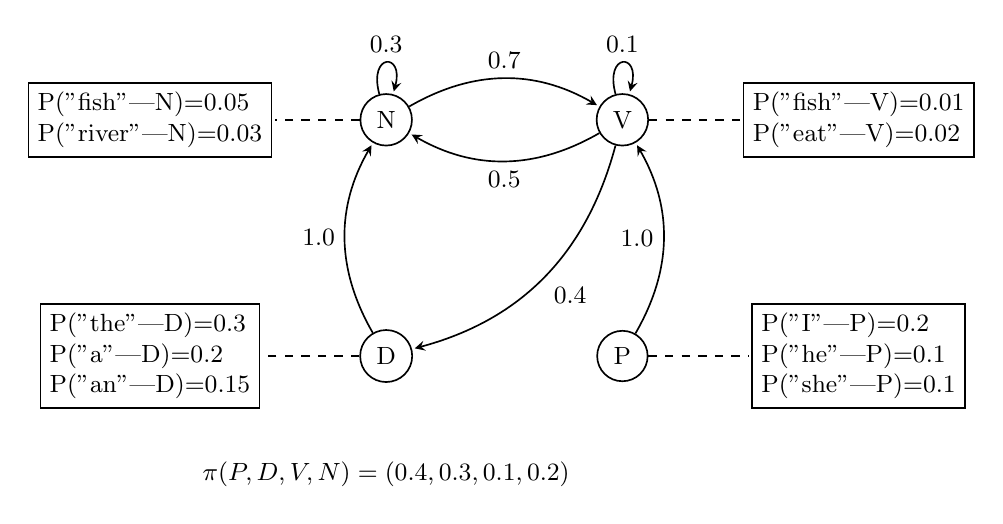
\begin{tikzpicture}[
		> = stealth, % arrow head style
		shorten > = 1pt, % don't touch arrow head to node
		auto,
		node distance = 3cm, % distance between nodes
		semithick, % line style
		font=\small
		]
		
		\tikzstyle{every state}=[
		draw = black,
		thick,
		fill = white,
		minimum size = 4mm
		]
		
		\node[circle,draw] (qN) {N};
		\node[align=left,draw] (qNe) [left of=qN] {P("fish"|N)=0.05\\P("river"|N)=0.03};
		\node[circle,draw] (qV) [right of=qN] {V};
		\node[align=left,draw] (qVe) [right of=qV] {P("fish"|V)=0.01\\P("eat"|V)=0.02};
		\node[circle,draw] (qD) [below of=qN] {D};
		\node[align=left,draw] (qDe) [left of=qD] {P("the"|D)=0.3\\P("a"|D)=0.2\\P("an"|D)=0.15};
		\node[circle,draw] (qP) [right of=qD] {P};
		\node[align=left,draw] (qPe) [right of=qP] {P("I"|P)=0.2\\P("he"|P)=0.1\\P("she"|P)=0.1};
		\node[] () [below of=qD, yshift=1.5cm] {$\pi(P, D, V, N) = (0.4, 0.3, 0.1, 0.2)$};
		
		\path[->] 	
		(qN) 	edge [loop above] node {0.3} ()
		edge [bend left] node {0.7} (qV)
		(qV) 	edge [loop above] node {0.1} ()
		edge [bend left] node {0.5} (qN)
		edge [bend left] node {0.4} (qD)
		(qD)	edge [bend left] node {1.0} (qN)
		(qP)	edge [bend right] node {1.0} (qV);
		
		\path[dashed] 	
		(qN) 	edge [] node {} (qNe)
		(qV) 	edge [] node {} (qVe)
		(qD) 	edge [] node {} (qDe)
		(qP) 	edge [] node {} (qPe);
		
	\end{tikzpicture}
	
	\begin{enumerate}
		\item Calculate the two probabilities: P(V D N | "fish a fish") and P(N D N | "fish a fish").
		\item Given that C(N) = 200, C(V) = 100, and C(D) = 100, calculate the following probabilities using Laplace smoothing: P(D|V), P(D|N), and P(N|D).
		\item Recalculate the probabilities from the first question after smoothing.
		\item How many expressions labeled "V D N" exist in our training dataset? The determinant "D" never occurs at the end of the sentence.
	\end{enumerate}
	
\end{enumerate}

%\end{resources}


\subsubsection*{Demos}

Demos are accessible via the Github repository.
In the first tutorial, we introduce the morpho-syntactic tagging task with NLTK, which is a Python-implemented tool for NLP. Several algorithms are used: RegEx, CRF, HMM, Perceptron, and Brill. We also present the named entity recognition task and the nominal phrase extraction task.

The second tutorial uses Flair, a Python tool for NLP. We cover both tasks: morpho-syntactic tagging and named entity recognition. In the tutorial, you can learn how to use an existing model and how to create a new one.

\subsubsection*{Lab: Morpho-syntactic Analysis}

We aim to design a small program for morpho-syntactic analysis from scratch. The HMM model with Laplace smoothing is provided. The student must implement the "Viterbi" decoding method.

The complete statement of the practical work along with the codes and data can be downloaded from the Github repository. The practical work is implemented entirely from scratch: the HMM module and the module that uses it for morpho-syntactic analysis. The student must complete two functions in the first module: scoring ($p(t_i|t_{i-1}, w_i)$) and Viterbi decoding. Two other decoding algorithms are implemented: brute force and greedy. The student must compare the three models by calculating the time complexity. The available programming languages (for now) are Java, Javascript/nodejs, and Python.


%\subsubsection*{Workshop}
%


%=====================================================================
\ifx\wholebook\relax\else
% \cleardoublepage
% \bibliographystyle{../use/ESIbib}
% \bibliography{../bib/RATstat}
	\end{document}
\fi
%=====================================================================
